\documentclass[11pt, preprint]{aastex}
%%%%%%begin preamble
\usepackage[hmargin=1.05in, vmargin=1in]{geometry} % Margins
\usepackage{hyperref}
\usepackage{url}
\usepackage{natbib}
\usepackage{graphicx}
\usepackage{amsmath}
\usepackage{amsfonts}
\usepackage{amssymb}
\usepackage{pdfpages} % breaks with aastex6
\usepackage{import}
\usepackage{wrapfig}

\usepackage{color}
\hypersetup{
  colorlinks   = true,
  %citecolor    = blue
  citecolor    = gray
  % gray is not being found!?!
  % gray is found if pdfpages is used... crap.
  %citecolor    = grey
  %citecolor    = Gray
}

\setcounter{tocdepth}{2}
%% headers
\usepackage{fancyhdr}
\pagestyle{empty}
\pagenumbering{gobble}
\renewcommand*{\thefootnote}{\fnsymbol{footnote}}

\renewcommand{\vec}{\ensuremath{\boldsymbol}}
\newcommand{\dedalus}{\href{http://dedalus-project.org}{Dedalus}}
\newcommand{\del}{\ensuremath{\vec{\nabla}}}
\newcommand{\scrS}{\ensuremath{\mathcal{S}}}

\newcommand{\nosection}[1]{%
  \refstepcounter{section}%
  \addcontentsline{toc}{section}{\protect\numberline{\thesection}#1}%
  \markright{#1}}
\newcommand{\nosubsection}[1]{%
  \refstepcounter{subsection}%
  \addcontentsline{toc}{subsection}{\protect\numberline{\thesubsection}#1}%
  \markright{#1}}

\usepackage{atbegshi}
%%%%%%end preamble


\begin{document}
\title{Convective Conundrums in the Asteroseismic Age:\\The interplay of rotation and magnetism in stellar convection}
\vspace{-0.5cm}
\maketitle

\vspace{-0.8cm}
\begin{flushleft}
  \textit{Principal Investigator:} Evan H. Anders 
\end{flushleft}

\vspace{-1.3cm}

\section{Motivation}
\sectionmark{Motivation}
\vspace{-6pt}

\paragraph{Asteroseismology}
\label{sct:asteroseismology}
The advent of asteroseismic science has closely paralleled that of exoplanetary science.
Early ground-based observations of stellar pulsations \citep[e.g.,][]{kjeldsen&frandsen1991, bouchy&carrier2001, bedding&all2001} have given way to datasets larger than $10^4$ stars \citep[e.g.,][]{yu&all2018, santos&all2019b} in the age of CoRoT, Kepler, and K2 data.
Another 20,000 asteroseismically-interesting targets are being observed in the TESS satellite's two-year mission \citep{schofield&all2019}.
By 2030 we expect to have observed $10^7$ pulsating red giants and $10^5$ dwarfs and subgiants \citep{huber&all2019}.
In addition to teaching us about the nature of stellar interiors, asteroseismology enables the accurate measurement of stellar ages, masses, and radii, which in turn facilitates studies in galactic archaeology and exoplanetary measurements.
Asteroseismic measurements generally rely on one-dimensional (1D) stellar structure models, and these models have some known deficiencies \citep{buldgen2019}, in particular their handling of three-dimensional (3D) dynamical phenomena like convection, rotation, and magnetism.
The exponential rise in asteroseismic targets demands a continued investment in the theory that informs these stellar models and asteroseismic measurements.

State-of-the-art stellar strucuture models are produced by 1D codes like MESA \citep{paxton&all2011}.
%The coupling of MESA models and the GYRE code \citep{townsend&teitler2013}, a stellar oscillation code which solves the linear equations governing stellar pulsations, has enabled efficient identification of pulsational modes in a wide variety of stars.
Unfortunately, MESA models necessarily depend on 1D parameterizations of convection and often employ the decades-old mixing length theory \citep[MLT,][]{bohm-vitense1958}.
While some aspects of convection are adequately described by MLT, it fails in a number of situations.
For example, 1D stellar models incorrectly produce pulsations in the surface layers of Sun-like stars, while 3D models of convection in these layers fare better \citep{jorgensen&weiss2019}.
%However, recent work suggests 1D interior models coupled with 3D simulations fare better when modeling these surface layers \citep{jorgensen&weiss2019}.
Additionally, 1D models assume spherical symmetry and generally neglect magnetic and rotational effects.
Observations of stellar flares \citep{kowalski2016} and magnetically-induced pulsational frequency shifts \citep{santos&all2018} suggest that magnetism should not be neglected.
%Recent work further suggests that the magnetic field topology impacts asteroseismic measurements \citep{thomas&all2019}, casting doubt on the efficacy of 1D models.
Furthermore, the Sun exhibits differential rotation characterized by latitudinal variations in angular velocity within the solar convection zone \citep{thompson&all1996, schou&all1998}, and latitudinal differential rotation has now been observed in other stars \citep{benomar&all2018}.
Together, these observations suggest that 1D parameterizations of convection which neglect complicating effects cannot sufficiently capture the complexities of stars.
In order to properly and fully utilize the large stores of incoming asteroseismic data, we must improve the models on which asteroseismic inversions rely.

\vspace{-0.5cm}
\paragraph{The Solar Convective Conundrum}
\label{sct:convective_conundrum}
The outer 30\% of the Sun is a highly stratified convective envelope, and recent observations reveal that we lack a fundamental understanding of dynamics in this region.
Various helioseismic observations \citep{hanasoge&all2012, greer&all2015} detect convective velocity magnitudes which are two orders of magnitude disparate.
Furthermore, these observations, as well as measurements of solar surface velocities \citep{hathaway&all2015}, have an unexpected absence of velocity at large spatial scales.
In short, we do not observe large-scale ``giant cells'' driven by buoyant motions deep in the solar convection zone.
These measurements, and the absence of giant cells, consitute the Solar Convective Conundrum.

Two primary hypotheses currently aim to explain the absence of giant cells: ``entropy rain'' and a rotationally constrained solar convective interior.
The entropy rain hypothesis, first suggested by \citet{spruit1997}, posits that theory over-predicts the importance of upflows and that \emph{downflows} are predominantly responsible for carrying the solar luminosity across the solar convection zone.
Recent theory and simulations, including some of my own work, suggest that small, intense downflows can indeed survive through the depth of the convection zone and may be more important than upflows in solar-like convection \citep{brandenburg2016, kapyla&all2017, andersLB2019}.
To date, this work neglects magnetism and rotation, and it is unclear how these complicating effects interact with these fast, powerful downflows.
Meanwhile, the rotationally constrained interior hypothesis suggests that Coriolis forces dominate the dynamics of deep solar convection, and that these forces mask giant cells.
Simulations by \citet{featherstone&hindman2016} show that as convective flows become more rotationally constrained, dominant convective velocities are pushed to smaller length scales.
However, rotational effects on simulations can be hard to quantify; some simulations which nominally rotate at the solar rate show \emph{anti-solar} differential rotation \citep{gastine&all2014}, and other rotationally constrained simulations exhibit Jupiter-like bands \citep{brun&all2017}.
Regardless, current results and hypotheses suggest that the interplay between downflows and rotational effects must be better understood in stellar convection.

\vspace{-0.5cm}
\paragraph{Modern convective simulations}
\label{sct:modern_simulations}
The earliest simulations in stellar-like convection \citep{graham1975, hurlburt&all1984, cattaneo&all1991, brummell&all1996, brummell&all1998} often sought to gain understand in simplified systems.
Cartesian geometry was employed, and convective flows in the presence of one or more complicating effects (stratification, rotation, magnetism, etc.)~were explored.
Despite vast modern computational resources, similar studies \citep[e.g.,][]{wood&brummell2012, anders&brown2017, wood&brummell2018} have become rare in the past two decades, and the highly laminar results of simulations from twenty years ago are often the state-of-the-art.

Recently, numericists have often switched aims from simply understanding convection to trying to reproduce precisely aspects of solar or stellar convection.
Large scale, ``global'' simulations of spherical rotating magnetoconvection exhibit cycling dynamos and latitudinal differential rotation \citep{brown&all2010, brown&all2011, guerrero&all2016, hotta&all2016, brun&all2017, strugarek&all2018}.
Small scale ``local'' simulations with realistic radiative transfer strikingly visually resemble solar surface convection and sunspots \citep{stein&nordlund1998, rempel&all2009, stein&nordlund2012, rempel2014}.
Local simulations have shaped how some observational experts interact with simulations, and the raw data of \citet{rempel2014}'s simulations are being used directly as high-resolution observations of solar convection \citep[see e.g.,][and others]{vankooten&cranmer2017, shchukina&trujillo2019}.
Unfortunately, simulations fail to reproduce some important aspects of solar convection \citep{hanasoge&all2015}.
Modern realistic simulations should partner with simplified setups, where effects like rotation and magnetism can be well understood, so that observational and theoretical discrepancies can be resolved.
This understanding can be employed to produce better ``realistic'' simulations which more accurately reflect aspects of true solar convection.
With a more detailed understanding of fundamental processes in stellar convection, realistic simulations can produce valuable synthetic observables for asteroseismologists, helioseismologists, and scientists who will soon use the NSF's Daniel K. Inouye Solar Telescope (DKIST) to study the solar surface at high resolution.


\section{Intellectual Merit}
\vspace{-6pt}
\sectionmark{Intellectual Merit}

\label{sct:intellectual_merit}

\paragraph{Rotating magnetoconvection across all scales}
Over the course of my postdoctoral studies, I will take advantage of the flexibility of the Dedalus pseudospectral framework \citep{burns&all2019}, which I have become proficient at using during my graduate career, to study numerical simulations at three different scales.
In task A, I will study simulations of discrete events, or thermals \citep[as in][]{andersLB2019}, which model individual stellar convective downflows and can achieve high levels of turbulence.
In task B, I will study simulations of mesoscale convection \citep[as in][]{anders&brown2017} to gain an understanding of how these effects behave in the presence of the convective-radiative interface at the base of a solar-like convective zone.
In task C, I will study simulations of global stellar convection \citep[as in][]{lecoanet&all2018}, developing and using new community tools to study the importance of rotation and magnetism over Kelvin-Helmholtz timescales.
Each task is expected to take one full year of my three-year postdoctoral fellowship.
%Over the course of these three tasks, I will aim to understand two fundamental questions.
%First, how do rotation and magnetism modify or constrain convective dynamics?
%Second, how do convective motions transport or generate angular momentum and magnetic fields?

\vspace{-0.8cm}
\subsection*{Task A: Dynamics of individual downflows}
\vspace{-0.3cm}
\label{sct:taskA}
\begin{wrapfigure}{l}{0.4\textwidth}
	\begin{center}
	\vspace{-10pt}
    \includegraphics[width=0.38\textwidth]{./figs/thermals_comparison.png}
	\vspace{-16pt}
	\end{center}
    \caption{
	3D visualizations of the entropy perturbation of evolved thermals in the laminar (left) and turbulent (right) regimes.
	\label{fig:thermals_comparison} }
\end{wrapfigure}

In the envelopes of lower main sequence stars, convection occurs in the presence of extreme stratification.
Stratified convection is characterized by powerful, localized downflows, and broad, slow upflows.
Recent theory and observations \citep[e.g.,][]{hanasoge&all2015, brandenburg2016, kapyla&all2017, andersLB2019} suggest that downflows may be the predominant mechanism for transporting stellar luminosity in these convective zones.
Furthermore, \citet{tobias&all1998} showed that downflows in convection can effectively pump magnetic fields downwards in certain regimes.
These results suggest that downflows in stratified convection deserve careful study.

Downflows may turbulently break up into distinct pieces as they fall and these pieces can be modeled as thermals.
Thermals are regions of cold fluid which accelerate due to buoyancy forces and shape themselves into vortex rings; evolved thermals are visualized in Fig. \ref{fig:thermals_comparison}.
Thermals are observed and studied in the Earth's atmosphere and are well understood in the Boussinesq limit.
%Recently, I studied thermals as a model for solar convection and came to understand the effects of stratification on the propagation of thermals \citep{andersLB2019}.

Thermals provide an excellent model of stellar downflows because they are relatively easy to model analytically and to simulate.
Hydrodynamic thermals in stratified domains have a solution which is essentially fully specified by: (a) the stratification of the background atmosphere and (b) whether they are laminar or turbulent.
Thanks to my work in \citet{andersLB2019}, the influence of stratification on thermals is now understood.
During my postdoctoral studies, I will study thermals in a fixed high-stratification regime and gain a theoretical and experimental understanding of the effects of magnetism and rotation on thermal evolution.
In a purely hydrodynamical context, \citet{lecoanet&jeevanjee2019} showed that turbulence does not appreciably change the evolution of thermals.
However, turbulence creates smaller scale structures in the propagating thermals which may be important in the context of rotation or magnetism.
Over the course of Task A, I will try to answer two fundamental questions about stellar downflows:
\vspace{-16pt}
\begin{enumerate}
\item Can stellar downflows transit the full depth of their convective envelopes, or do rotational or magnetic processes inhibit their propagation?
\vspace{-10pt}
\item How much energy do downflows transport, and in which regimes do rotational and magnetic effects change their energy fluxes?
\vspace{-10pt}
\end{enumerate}

\vspace{-0.5cm}
\paragraph{Task A.1: Rotational filtering of downflows}
\label{sct:taskA1}
In order to study the effects of rotation, I will study thermals in simple Cartesian domains.
These plane-parallel atmospheres exist at a fixed latitude and experiencing Coriolis forces from a global rotation rate.
I propose to study downflows at the equator, poles, and mid-latitudes.
At each of these latitudes, I will study flows which experience varying degrees of rotational constraint.
I will initially study laminar thermals to understand parameter space, but will later examine select turbulent simulations in all regimes which exhibit distinctly different behavior.
The primary goal of these studies will be to determine at which latitudes, and at which degrees of rotational constraint Coriolis forces prevent thermals from transiting the convection zone.
Understanding these questions will help constrain the effect of stellar rotation on how much energy downflows can transport.

\vspace{-0.5cm}
\paragraph{Task A.2: Magnetic filtering of downflows}
\label{sct:taskA2}
I will secondarily study thermals in the presence of magnetism but absence of rotation.
The inclusion of magnetism requires a choice of initial magnetic field setup, and I will study both cases in which there is a uniform background field and where there is a thin horizontal sheet of magnetism for the thermal to pass through \citep[as in][]{tobias&all1998}.
I will vary the orientation of the initial magnetic fields and the strength of magnetic forces on the flows, in a manner analagous to the rotational simulations in Task A.1.
This work will be the magnetic complement to Task A.1, further constraining regimes in which downflows can effectively propagate through a stellar convection zone to transport the stellar luminosity.


\vspace{-0.8cm}
\subsection*{Task B: Mesoscale interactions at the radiative-convective boundary}
\vspace{-0.3cm}
\label{sct:taskB}
\begin{figure*}[t!]
    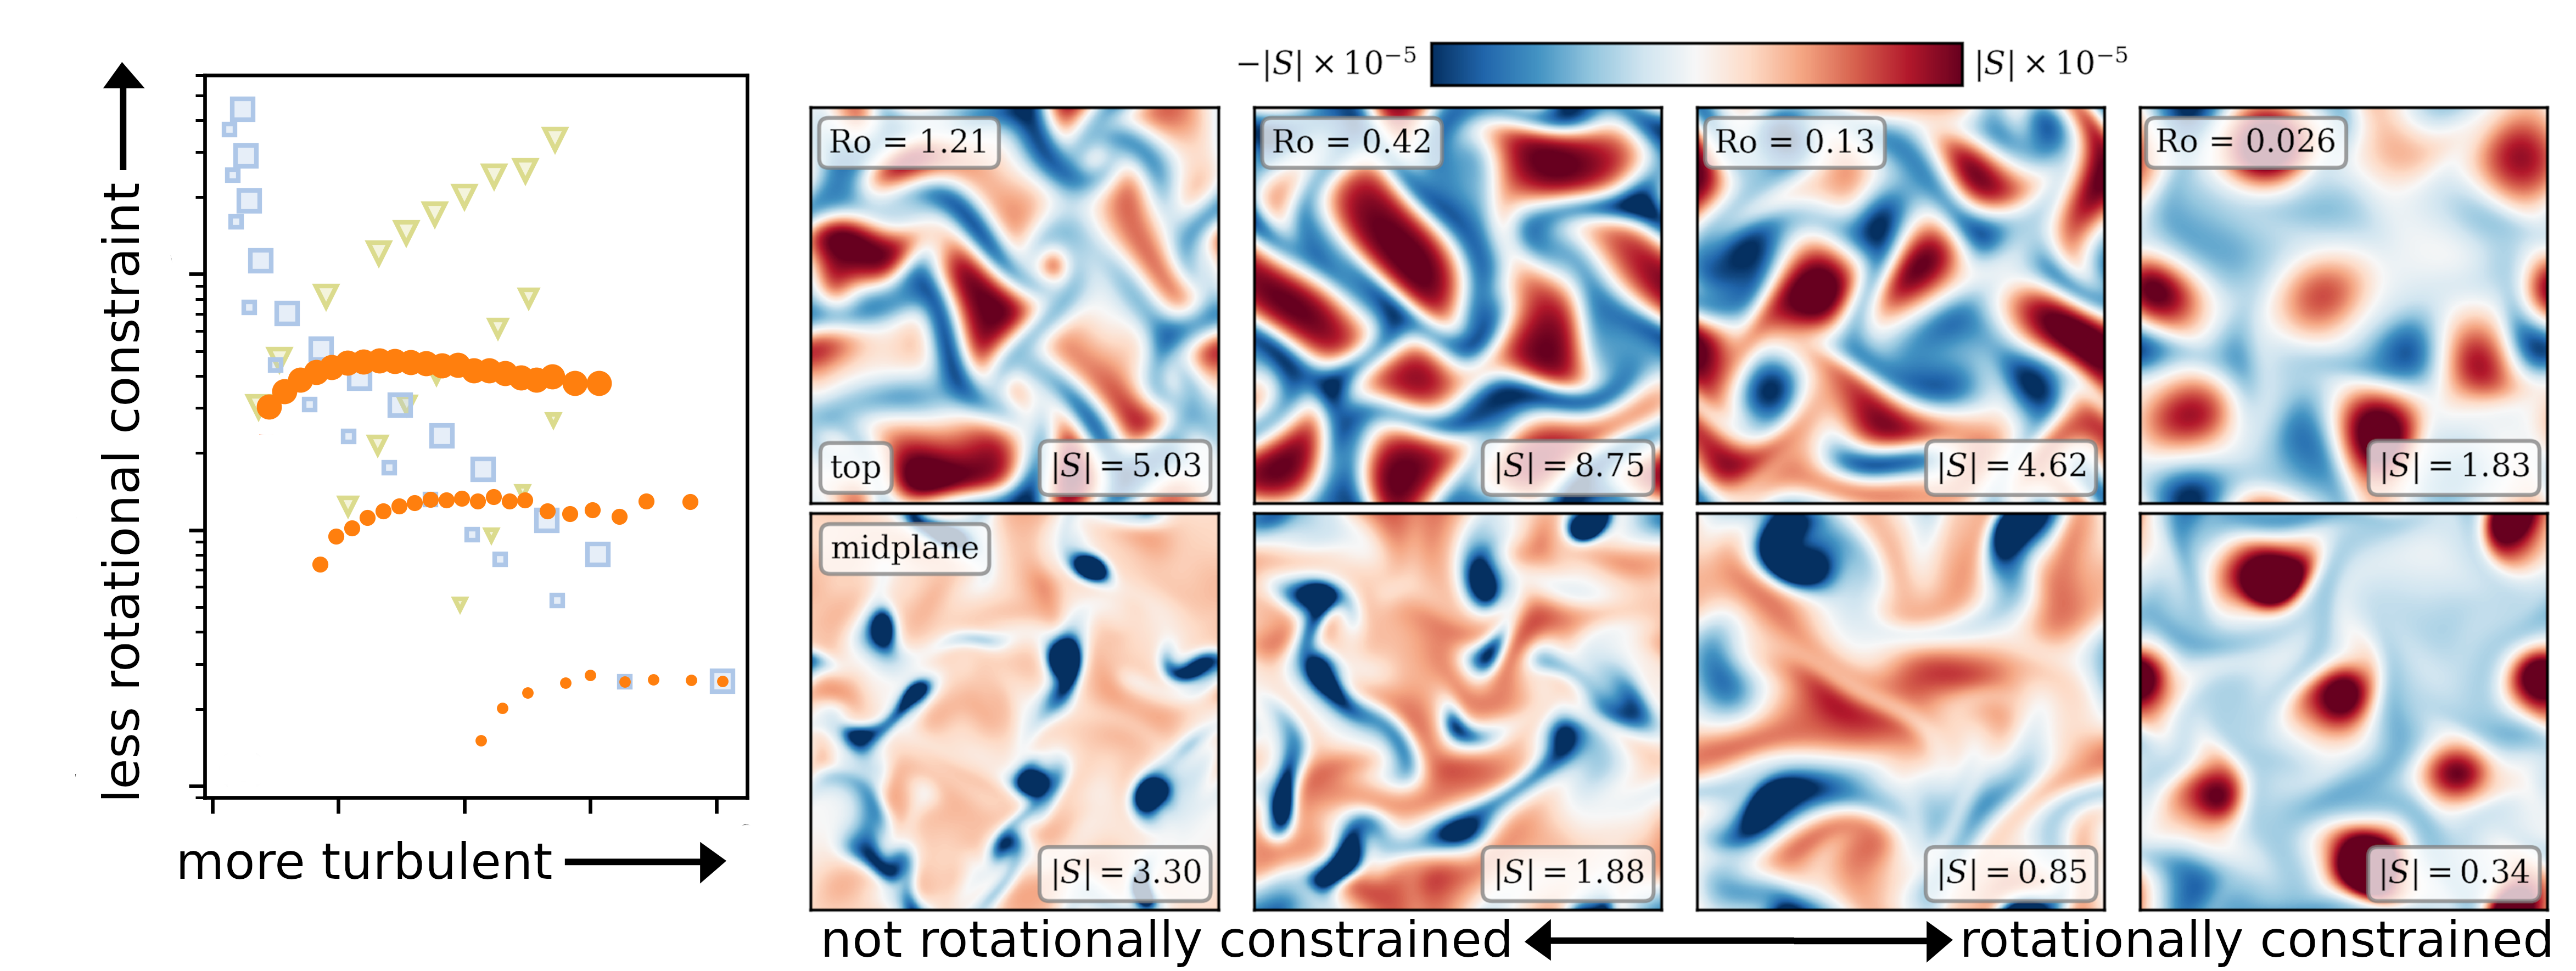
\includegraphics[width=\textwidth]{./figs/rossby_plot.png}
    \caption{(left, Fig 1b of \citet{anders&all2019}) The degree of rotational constraint is difficult to predict as a function of turbulence in convective simulations.
	Along traditional paths through parameter space (green triangles and blue squares), rotational constraint varies strongly as a function of turbulence.
	However, when our newly discovered ``predictive Rossby number'' is held constant (orange circles), the degree of rotational constraint can be held constant while turbulence is increased.
	(right eight panels, Fig. 2 of \citet{anders&all2019}) As rotational constraint increases (from left to right), traditional granular convective patterns give way to quasi-two-dimensional vortical columns of convection with very little difference between the top of the atmosphere and the atmospheric midplane (top row vs. bottom row).
	Rotational constraint modifies convective dynamics, so simulating in the proper rotational regime that reflects the Sun or another star being studied is crucial.
	\label{fig:rossby_plot} }
\end{figure*}

In solar-like stars, the strongly stratified convective zone overlies a stable interior radiative zone.
In the Sun, the radiative-convective boundary (RCB) is characterized by a transition from moderate instability to strong stability.
Now that downflows are considered a crucial element of stellar convection, it is crucial to understand how these downflows interact with the RCB.

Helioseismic measurements suggest that the RCB is thin -- roughly 5\% of a pressure scale height at the base of the convection zone, or 1\% of a solar radius \citep{basu1997}.
However, dynamics in simulations rarely achieve such a thin RCB, often times producing RCB thicknesses which are too thick or too thin by up to an order of magnitude \citep[see e.g.,][]{hotta2017, kapyla2018}.
This suggests that simulations of stellar convection are in the wrong stiffness regime \citep{brummell&all2002, couston&all2017}.
Furthermore, magnetism can appreciably alter deep velocity magnitudes, which can in turn affect RCB thicknesses \citep{hotta&all2015}.
It is widely thought that dynamics in the RCB are a critical ingredient in generating the solar dynamo and magnetic field, and so understanding the effects of a too-thick or too-thin RCB is crucial.
I propose studying how the stiffness of the RCB, which determines how hard of a ``wall'' convective motions hit at that interface, affects the transport of angular momentum and magnetic fields into the radiative zone by downflows.
I will only conduct these simulations in flow regimes where downflows can feasibly transit the solar convection zone, as determined by Task A.
In those regimes, the goal of this task is to determine how angular momentum and magnetism are pumped into the RCB as a function of RCB stiffness.

\vspace{-0.5cm}
\paragraph{Task B.1: The critical magnetic field}
\label{sct:taskB1}
Convection in the presence of a strong magnetic field will have dynamics which are strongly affected by that field.
Similarly, a weak magnetic field will not noticeably affect convective motions.
There is therefore a critical field strength at which convection passes from being weakly to strongly affected by magnetism.
Observationally, one would expect stars with more vigorous convection to have a higher critical field strength, and hotter stars will likely have more vigorous convection and higher critical field strengths.
Unfortunately, the mapping of this intuition to simulations is not straightforward, and it is difficult to predict simulation flow regimes \emph{a priori}.
The goal of this task is to determine the critical field strength.

In rotating convection, an analagous argument can be made, where convection in the presence of rapid rotation is strongly affected by Coriolis forces, and this is not true in the presence of slow rotation.
During my graduate career, I identified the critical angular velocity in convective simulations, analagous to the critical magnetic field I am searching for here \citep[][and Fig. \ref{fig:rossby_plot}]{anders&all2019}.
Using similar methods to this work, I will determine the critical magnetic field strength in these mesoscale simulations.
Understanding the critical magnetic field and angular velocity will enable the stellar modeling community to more accurately study convection with proper force balances.

\vspace{-0.5cm}
\paragraph{Task B.2: Downflow interactions at the RCB}
\label{sct:taskB2}
In this task, I will study how downflows pump angular momentum and magnetism into or across the RCB.
I will study both very stiff RCBs, which act similar to hard wall boundaries, and very soft RCBs which convective motions can easily pass through.
Using this knowledge gained in task B.1, I will study simulations of convection in the magnetic and rotational regimes where task A revealed that downflows could transit the full convection zone.

\citet{tobias&all1998} showed that convective motions can effectively pump magnetic fields across soft RCBs in certain parameter regimes.
Here I will extend that work  to determine if magnetic fields and angular momentum are capable of being pumped into stiff RCBs by convective motions.
It is widely believed that shearing motions in the solar RCB are a critical piece of the solar dynamo, but observations \citep{basu1997} suggest that the solar RCB is stiff.
If convective motions are not able to pump magnetic fields into a stiff RCB, then a different mechanism must be responsible for generating new magnetic fields.
Furthermore, a stiff RCB could potentially insulate the solar radiative interior from convectively-driven angular momentum transport, which could help explain why the solar differential rotation profile gives way to a uniformly rotating interior beneath the RCB.

\vspace{-0.8cm}
\subsection*{Task C: Global studies in relaxed atmospheres}
\vspace{-0.3cm}
\label{sct:taskC}

\begin{wrapfigure}{r}{0.3\textwidth}
	\begin{center}
	\vspace{-10pt}
    \includegraphics[width=0.28\textwidth]{./figs/mdwarf.png}
	\vspace{-16pt}
	\end{center}
    \caption{A volume rendering of a global dynamo simulation in Dedalus.
	Enstrophy, or the magnitude of vorticity, is shown in green.
	Red and blue lines denote the magnitude and direction of azimuthal magnetic field.
	\label{fig:mdwarf} }
\end{wrapfigure}

The capstone project of my postdoctoral studies will study convection at the largest scales: global spherical simulations of rotating magnetoconvection.
The tools to perform these simulations in Dedalus already exist \citep{lecoanet&all2018} and have been tested; a visualization of basic outputs from these simulations is shown in Fig. \ref{fig:mdwarf}.
One major barrier to performing turbulent global simulations is that they are costly, and some of these costs are unavoidable: highly resolved, turbulent simulations necessarily take small timesteps, and therefore simulation times are very long.
However, some of the expense of these simulations is often time wasted waiting for the atmospheric structure and mean flows to converge to an equilibrium state.
For example, the thermal structure of the Sun is thought to evolve over its Kelvin-Helmholtz timescale of $10^7$ years, which is significantly longer than its convective overturn time of five minutes at the solar surface, although still much shorter than its main sequence lifetime \citep{anders&all2018}.
As simulations approach the turbulent regime of stars, relaxation and dynamical timescales become extremely disparate, and in general numericists must choose between having state-of-the-art turbulence or converged, statistically equilibrium dynamics -- but not both.
During this third task, I will develop, test, and utilize a community tool which effectively establishes mean flows and evolves atmospheric structures by taking much larger timesteps than those of convection.
By doing so, I will enable global dynamo simulations which are both in thermal equilibrium and exhibiting state-of-the-art turbulence.


During my graduate career, I studied a mechanism for accelerating the long thermal relaxation timescale in convective systems \citep{anders&all2018}.
In this work, we discovered that a tool like the one I am proposing here can be feasibly implemented and tested for accuracy.
While studying turbulent flows, we found that our tool reached a relaxed state using an order of magnitude fewer computational resources than when waiting for a standard thermal relaxation timescale.
These speedups make achieving thermal relaxation in state-of-the-art simulations feasible.

\vspace{-0.5cm}
\paragraph{Task C.1: Accelerated evolution of global simulations}
\label{sct:taskC1}
During my postdoctoral studies, I will extend my accelerated evolution method to the evolution of thermodynamic and angular momentum profiles in global simulations.
The development of this extension will be grounded in understandings gained in tasks A and B.
In particular, task A will inform which terms in the equations importantly adjust the mean field in certain regimes, and task B will inform how to implement this technique near RCB-like interfaces.
As I did in \citet{anders&all2018}, I will verify that this method produces the same results as a long relaxation in modest parameter regimes to build trust in the method.
This module will be made public, and will be designed so as to flexibly interact with arbitrary simulation data so that users of codes beyond Dedalus can benefit from the computational speed-ups of this tool.

\vspace{-0.5cm}
\paragraph{Task C.2: Relaxed simulations of the solar dynamo}
\label{sct:taskC2}
I will study simulations of the interior solar convection zone in regimes where flows feel the effects of both rotation and magnetism, using the knowledge from task B.1 to determine how to set up such simulations.
Using the tool developed in task C.1, I will accelerate the evolution of these simulations.
I am predominantly interested in the relaxed differential rotation profiles that appear as a function of rotational constraint, and how these differential rotation profiles affect the time evolution of the magnetic dynamo.
In most modern dynamo simulations, the evolution of magnetic fields are measured during the relaxation process, and it is possible that the time-dependent dynamo behavior of the simulation is strongly influenced by the underlying evolution of the mean state.

While these simulations will be largely targeted in the solar context, the accelerated evolution tools which will be developed and tested here could have great benefits for asteroseismic research.
Recently, \citet{jorgensen&weiss2019} coupled 3D, global simulations with 1-dimensional stellar structure tools in order to more accurately produce stellar structure profiles to great success.
The fast equilibration of angular momentum and thermal profiles described here is essentially equivalent to taking timesteps which superstep the convective motions, similar to those taken in any 1D stellar structure model.
Put simply, these accelerated evolution techniques would be a first step to enabling a generalized coupling of 1-dimensional stellar structure codes with realistic statistics from converged global convection.
Future asteroseismic inversions will then benefit from stellar structure models which are influenced by 3D convection including complicating effects like magnetism and rotation.

\vspace{-0.8cm}
\subsection*{Computational Feasibility}
\vspace{-0.3cm}
\label{sct:feasibility}
Tasks A-C are arranged logically from smallest to largest scales, and also from least to most computationally expensive.
Based on the work in \citet{anders&brown2017, anders&all2018, anders&all2019, andersLB2019}, Dedalus takes $\mathcal{O}(10^3)$ cpu-sec per iteration for a run with a grid resolution of 384$^3$ on a system comparable to NASA Pleiades.
Task A runs of thermals will take $\mathcal{O}(10^4)$ iterations each, while turbulent runs in tasks B and C will take $\mathcal{O}(10^6)$ iterations each.
Laminar thermal simulations thus cost roughly 5000 cpu-hours each, while turbulent thermals cost roughly $10^5$ cpu-hours each.
State-of-the-art simulations in tasks B and C will cost roughly $10^6$ cpu-hours each.
The projects described here total 5-10 million cpu-hours per year in tasks B and C, with less (2-3 million cpu-hours) in the first year while thermals are being studied.

The computational cost of task A should be feasible to obtain on Northwestern's 11,800-core Quest supercomputer.
In order to increase my access to computational resources and to allow for larger scale runs in tasks B and C, I will leverage my AAPF fellowship and apply for time on NSF XSEDE resources such as Stampede2, Comet, or Bridges.


\vspace{-0.8cm}
\subsection*{Collaborative studies at CIERA}
\vspace{-0.3cm}
\sectionmark{CIERA}
\label{sct:ciera}
Northwestern university, and specifically the Center for Interdisciplinary Exploration and Research in Astrophysics (CIERA), is the perfect location for me to carry out the work proposed here.
Prof.~Daniel Lecoanet, who will be my primary advisor and collaborator, is one of Dedalus' founders.
His expertise using Dedalus and his past work on thermals \citep{lecoanet&jeevanjee2019, tarshis&all2018}, convection \citep{lecoanet&quataert2013, lecoanet&all2014, couston&all2017}, rotating convection \citep{couston&all2019}, and global simulations \citep{lecoanet&all2018} will make him a valuable collaborator and advisor for the projects proposed here.
Furthermore, I have already published a paper on thermals in close collaboration with Prof.~Lecoanet \citep{andersLB2019}, so task A will serve as an excellent transition project into my postdoctoral studies on my arrival.
In addition to Prof.~Lecoanet, Prof.~Yoram Lithwick would be an excellent partner for collaboration due to his past work on rotating convection \citep{BDLithwick2014} and his continuing collaborations studying careful and numerical problems in fluid disks \citep{LDLithwick2019} and planetary systems \citep{hadden&lithwick2018}.
CIERA houses many experts in computational fluid dynamics beyond Profs.~Lecoanet \& Lithwick, such as Profs.~Sasha Tchekhovskoy \& Claude-Andre Faucher-Giguere.
I look forward to joining the astrophysical fluid dynamics group at CIERA where I will have many opportunities to discuss and develop new numerical techniques, strategies, and applications across astrophysics.


Furthermore, in addition to the focused educational and outreach projects described below in section \ref{sct:broader_impacts}, CIERA will provide me with numerous small scale opportunities to participate in public outreach.
CIERA's Astronomy on Tap program as well as its CIERA Astronomer Evenings provide bite-sized and accessible ways to interact with the public.
Dearborn Observatory's observation tours are very similar to the public open houses I helped host at CU Boulder's Sommers-Bausch observatory.
The state-of-the-art Adler planetarium also provides similar opportunities such as its \emph{`Scopes in the City} program or its Space Visualization Lab astronomy conversations.
This program aligns with NSF broader impact goals in a couple of ways.
First, it improves STEM educator development at two levels: young career scientists (graduate students) and high school educators.
Second, it widely increases public engagement with authentic science at the high school level through the wide deployment of these modules.


\section{Broader Impacts}
\vspace{-6pt}
\sectionmark{Broader Impacts}
\label{sct:broader_impacts}

\paragraph{Motivation}
A majority of high school students across Illinois and in the Chicago area are not meeting science and math standards.
In 2017-2018, only roughly 40\% of students at the high school level were proficient on the Illinois Science Assessment and fewer were considered proficient on their math SAT scores \citep{irc2018}.
While on average these outcomes are slightly better in Chicago schools than Illinois as a whole, many Illinois and Chicago schools with higher poverty concentrations score lower than these state-wide averages \citep{stevens&all2015}.  
Numerous outreach activities which involve short-lived visits to high schools aim to address these problems and seem to positively improve STEM attitudes and engagement at the high school level \citep{vennix&all2017, vennix&all2018}.
Secondary teacher feedback regarding these programs suggests that one of the crucial features of effective outreach programs is the expertise of the visiting scientists on the topics they teach \citep{laursen&all2007}.

At the university level, common practices in physics education are being researched and reconsidered.
The norm in our field has been to teach physics predominantly through lectures, but evidence is now showing that students learn less in these standard courses than we assume and the use of alternate modes of instruction can improve learning outcomes \citep{meltzer&thornton2012}.
In addition to struggling to impart knowledge, these traditional course methods often lead to regression of student attitudes regarding science towards less favorable responses from the beginning to the end of introductory courses \citep{reddish&all1998}.

Science education clearly faces struggles in achieving desired outcomes at both the secondary and collegiate level.
However, improved STEM engagement has been seen at the secondary level when topical experts are involved in course module design, and improved physics learning and engagement have been measured at the university level when modern teaching pedagogical techniques are acknowledged and applied.
During my time at CIERA, I will bring together local experts on teaching pedagogy (high school teachers) and physics (graduate students at CIERA) to improve learning outcomes at the secondary and post-secondary levels.

\vspace{-0.5cm}
\paragraph{Improving physics education outcomes through collaborative sharing of expertise}
I propose the creation of a workshop series which partners scientific and pedagogical experts.
Over the course of this workshop series, pedagogically- and scientifically- sound teaching modules will be built that can be used in high school classrooms across the Chicago area and the nation.
At the start of this workshop series, the specific learning outcomes of these modules will be specified by our pedagogical experts using Next Generation Science Standards (NGSS) disciplinary core ideas in physics.
Our pedagogy experts will identify these topics as areas where their students struggle to learn, where they would like to work collaboratively with a topical expert to design a new lesson plan.
Small groups consisting of at least one pedagogical and scientific topical expert will be formed around each module.
During the development of each course module, an NGSS scientific practice, such as planning and carrying out investigations, will also be chosen by the group to incorporate into the module so that students have opportunities to participate in scientific practices as well as learn scientific ideas.

This workshop series will meet once or twice a week for 2-3 hours apiece over the course of a ten-week time interval.
Individual workshop meetings will consist of a large-group lesson in teaching pedagogy, followed by small-group work on module development in which that pedagogical lesson is applied.
This format will enable graduate student participants to learn pedagogical lessons and then immediately see them applied while they gain an understanding of the intricacies of curriculum design.
%This format will further ensure that each module lesson is built from the ground up, with careful attention and expertise on both the subject matter and practical applicability in the classroom.

These workshops will expose young career scientists to some basic teaching pedagogical research which they will be able to employ at the university level in their careers.
Furthermore, these workshops will expand the scientific content knowledge of participating high school teachers in a self-identified area of teaching difficulty.
On a larger scale, this program will produce well-informed teaching modules which can be used widely in high schools, and will leverage connections and input from high school teachers to help ensure adoption of these modules in the classrooms.

\vspace{-0.5cm}
\paragraph{Collaborative development}
\label{sct:development}
Participation from educators will be crucial for the success of the program proposed here.
I will partner with local teacher organizations such as Physics Northwest, the Illinoise State Physics Project (ISPP), and the Chicago Section of the American Association of Physics Teachers (CSAAPT).
Physics Northwestern's monthly meetings, ISPP's quarterly meetings, and CSAAPT's biannual meetings will be excellent venues in which to advertise the program and build a professional network of interested educators in the Chicago area.
Furthermore, CIERA's \emph{Reach for the Stars} program, an NSF GK-12 program, has partnered with many local area high schools over the past decade and will serve as an excellent in-house link to this audience.
In addition to working with local high school educators through these avenues, I will reach out to experts in Northwestern University's School of Education and Social Policy to enlist their assistance in the development of my workshop series.

While building up these cross-disciplinary collaborations, I will work alongside Ms. Michelle Paulsen, CIERA's Director of Education, Outreach, and Communications Programs, to develop my workshop series.
Ms.~Paulsen has experience as a high school physics teacher and has been the chair of a large suburban high school's science department.
Furthermore, Ms.~Paulsen has been instrumental in the creation of CIERA's RCTP program, which develops the presentation skills of young career scientists and includes cross-disciplinary collaborations and a ten-week workshop series similar to the one I propose here.
This workshop series will take place during the summer quarter, at a time when high school educators and graduate student schedules are not constrained by the school year.

The capstone of this workshop series for educators will be the production and use of these modules in their own classrooms.
However, graduate student participants do not have classes of students to return to with this content.
Fortunately, CIERA has a close connection with the Chicago Public Library system, and CIERA graduate students are already running data science clubs for interested area high school students.
I will work with the library, CIERA, and these data science clubs to create a venue where graduate student graduates of this program can teach these modules to interested students.

\vspace{-0.5cm}
\paragraph{Module distribution \& workshop outcomes} 

While these modules will naturally be implemented in the classrooms of the teachers who participate in this workshop series, I will work to ensure further distribution of these modules.
In my later years at CIERA, in addition to using connections with Physics Northwestern, ISPP, and CSAAPT to foster educator excitement in this program, I will use these avenues to advertise the specific modules that have been created.
They will be made publically available on the American Association of Physics Teachers online ComPADRE system, which stores resources for physics and astronomy educators and is publically available.
These modules will also be made available on CIERA's website, just as products from current programs like \emph{Reach for the Stars} are.
 \vspace{2pt}\\
In summary, this workshop series will: 
\vspace{-14pt}
\begin{enumerate}
\item Expose interested graduate students at CIERA to best practices in teaching pedagogy, and provide those students with a teaching experience.
\vspace{-9pt}
\item Expand content knowledge of high school educators while providing them with a strong lesson plan to employ on a topic that their students struggle to learn.
\vspace{-9pt}
\item Connect university scientists with teachers and teaching organizations in the greater Chicago area to create lasting partnerships between scientific and pedagogical experts.
\vspace{-9pt}
\item Distribute widely applicable teaching modules appropriate to the high school level which simultaneously teach core ideas and scientific practices, as defined by Next Generation Science Standards (NGSS).
\vspace{-9pt}
\end{enumerate}




\section{Personal career growth and development}
\vspace{-6pt}
\label{sct:personal_growth}
My graduate education has given me numerous opportunities to develop as a researcher, a teacher, and a member of my workplace community; see my biographical sketch for a brief description of some of these experiences.
These experiences have given me confidence that I enjoy teaching and research equally, and have affirmed my career goal to become a professor at the university level.
My proposed activities build naturally on research, outreach, teaching, and professional development work that I carried out as a graduate student, and will be feasibly accomplished over the next three years.
I will continue my development as a researcher through carrying out the work described in section \ref{sct:intellectual_merit}.
Furthermore, I will strive to expand my research network over the course of my postdoctoral research, and working with Prof.~Lecoanet will enable me to form many valuable connections within CIERA and across the nation.
My development as a teacher will be continued through the implementation of the workshop series described in section \ref{sct:broader_impacts}, and I am excited about the opportunity to learn personally from pedagogical experts while developing and facilitating this program.

\section{Summary and Perspectives}
\vspace{-6pt}
Observations of pulsating stars are plentiful but require 1D models which depend upon simple parameterizations of convection.
Unfortunately, observations of the Sun have revealed that our parameterizations and fundamental understanding of stellar convection are flawed.
Numerical simulations have been useful tools for establishing our understanding of stellar convection or modeling observations, but modern simulations are often overly complex and partnerships between complex and simplified systems should be used to understand these troubling observations.

The simulations proposed here are necssary and timely.
Current convective models cannot explain the Convective Conundrum and the combined effects of downflows, rotation, and magnetism is unclear and has not been well explored.
An understanding of these effects can help improve the underlying stellar structure models used in the ever-growing field of asteroseismology.
Furthermore, these studies will ensure that convective models accurately model flows in the stellar regime, which is crucial at a time when simulations are increasingly being treated as obervations.
The fundamental problems presented here are of broad scientific interest, but are specifically topics of NSF investigation, as evidenced by the NSF's support for the DKIST telescope which will soon come online.
The collaborative studies centered at CIERA will address the following key questions:
\begin{itemize}
\vspace{-9pt}
\item How strong do rotation and magnetism have to be to prevent entropy rain -- and stellar downflows -- from being a dominant dynamical process?
\vspace{-9pt}
\item Is the interaction of downflows with the radiative-convective boundary responsible for stellar differential rotation and stellar magnetic dynamos?
\vspace{-9pt}
\item What rotational regime reproduces the solar differential rotation profile, and what type of dynamo does that profile produce in a relaxed simulation? 
\vspace{-9pt}
\end{itemize}

Task A will occupy my research time during my first year; during this time I will also establish (fall through spring quarter) and teach (summer quarter) the first iteration of my teaching workshop series.
Task B will occupy my time during my second year, during which time I will iterate upon my workshop series and advertise the products of the first series. 
I will cap off my time at CIERA with task C while I work to ensure that my program transitions to new leadership when I leave so that future students can continue to reap its benefits.


\newpage
\AtBeginShipout{%
\AtBeginShipoutDiscard
}
\setcounter{page}{1}
\nosection{References}
\bibliographystyle{apj_title}


%\newpage
%\bibliographystyle{apj_title}
\bibliography{biblio}
\end{document}
